
\section{Web Search}

\begin{breakbox}
\boxtitle{Evaluating IR System:}
\begin{itemize}
	\item Note: the information need is translated into a query.
	\item Query: wine red white heart attack effective.
	\item Relevance is assessed relative to the information need not the query.
	\item E.g., Information need: I'm looking for information on whether drinking red wine is more effective at reducing your risk of heart attacks than white wine.
	\item You evaluate whether the doc addresses the information need, not whether it has these words.
\end{itemize}
\end{breakbox}

\begin{breakbox}
\boxtitle{Precision \& Recall:}
\newline Confusion Matrix:
\begin{center}
\begin{tabular}{| l | l | l |}
\hline
 & Relevant & Nonrelevant \\ \hline
Retrieved	& True pos. (tp) & False pos. (fp) \\ \hline
Not Retrieved & False neg. (fn) & True neg. (tn) \\
\hline
\end{tabular}
\end{center}
\begin{itemize}
	\item Precision $= \frac{tp}{(tp + fp)} = \frac{\text{\# (found and relevant)}}{\text{\# found}}$
	\item Recall $= \frac{tp}{(tp + fn)} = \frac{\text{\# (found and relevant)}}{\text{\# relevant}}$
\end{itemize}
\begin{center}
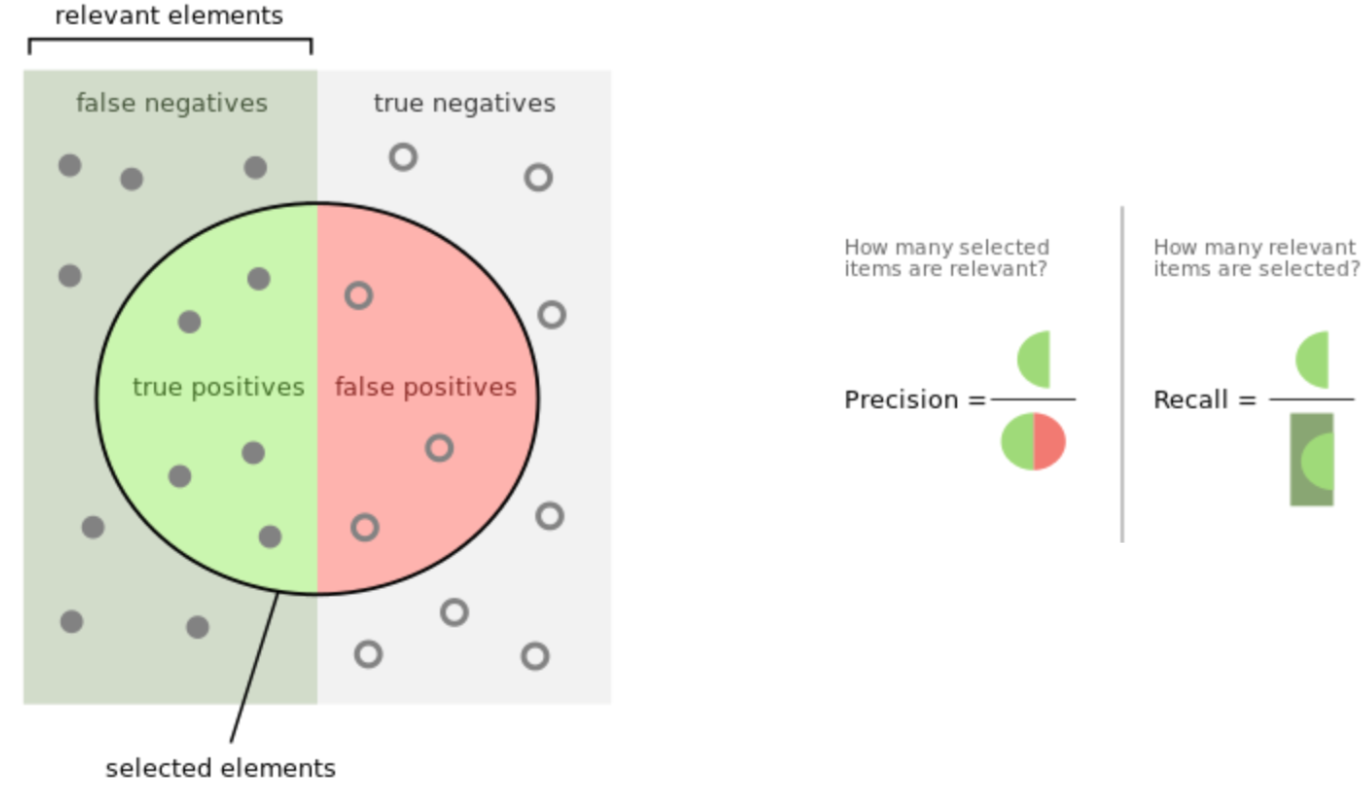
\includegraphics[width=.15\textwidth]{slides_images/precision_recall}
\end{center}
\end{breakbox}

\begin{breakbox}
\boxtitle{Notes:}
\begin{itemize}
	\item You can get high recall (but low precision) by retrieving all docs for all queries!
	\item Recall is a non-decreasing function of the number of docs retrieved
	\item In a good system, precision decreases as either the number of docs retrieved or recall increases.
\end{itemize}
\end{breakbox}

\begin{breakbox}
\boxtitle{Difficulties With Recall:}
\begin{itemize}
	\item Relevant docs. in doc. pool and relevant retrieved docs. From query: impossible!
	\item Should average over large document collection/query ensembles.
	\item Need human relevance assessments.
	\item Assessments have to be binary.
	\item Heavily skewed by collection/authorship.
	\item It is nearly impossible to calculate recall for web.
\end{itemize}
\end{breakbox}

\begin{breakbox}
\boxtitle{Precision/Recall Curve:}
\begin{center}
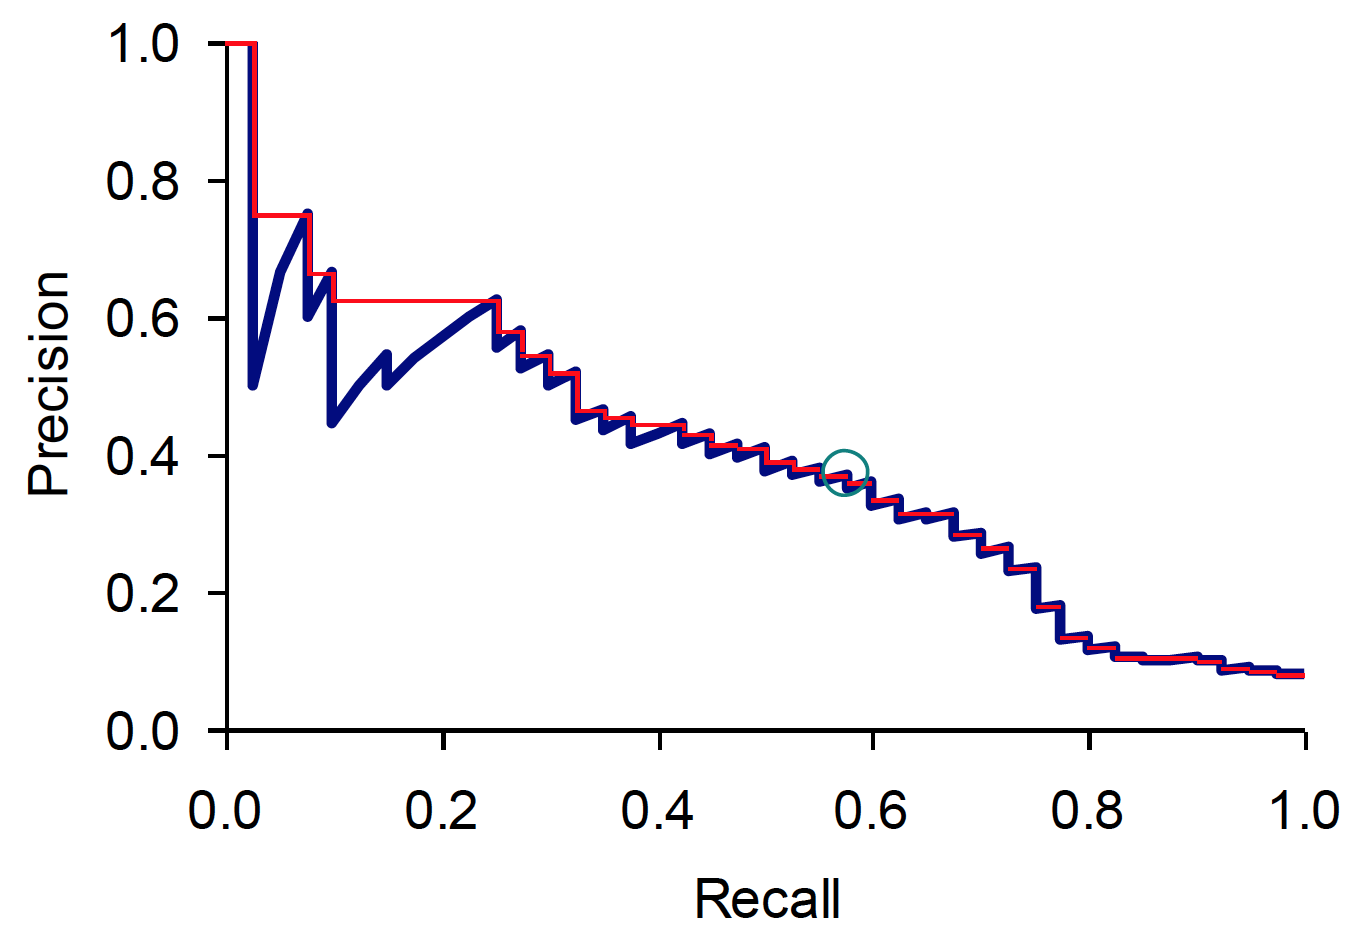
\includegraphics[width=.15\textwidth]{slides_images/precision_recall_curve}
\end{center}
\end{breakbox}

\begin{breakbox}
\boxtitle{A/B Testing:}
\begin{itemize}
	\item Purpose: Test a single innovation.
	\item Prerequisite: You have a large search engine up and running.
	\item Have most users continue to use the old system.
	\item Divert a small proportion of traffic (e.g., 1\%) to the new system that includes the innovation.
	\item Evaluate with an automatic measure like clickthrough-rate on first result.
	\item Now we can directly compare if the innovation does improve user happiness.
	\item Probably the evaluation methodology that large search engines trust most (def. used by Google).
	\item In principle this is less powerful than doing a multivariate regression analysis, but easier to understand.
\end{itemize}
\end{breakbox}



















